% Chapter 1

\chapter{Introducción general} % Main chapter title

\label{Chapter1} % For referencing the chapter elsewhere, use \ref{Chapter1} 
\label{IntroGeneral}

%----------------------------------------------------------------------------------------

% Define some commands to keep the formatting separated from the content 
\newcommand{\keyword}[1]{\textbf{#1}}
\newcommand{\tabhead}[1]{\textbf{#1}}
\newcommand{\code}[1]{\texttt{#1}}
\newcommand{\file}[1]{\texttt{\bfseries#1}}
\newcommand{\option}[1]{\texttt{\itshape#1}}
\newcommand{\grados}{$^{\circ}$}

%----------------------------------------------------------------------------------------

%\section{Introducción}

%----------------------------------------------------------------------------------------
El capítulo presenta las necesidades a satisfacer y una introducción técnica breve, con el objetivo de proveer los conceptos necesarios para comprender el resto de la memoria.

\section{Motivación}
\label{ch1Motivacion}

La tendencia tecnológica actual es interconectar los dispositivos a través de la Internet, a tal punto que la cantidad de objetos en el año 2009 superó al número de personas conectadas, y llegado el 2020 la diferencia es de seis veces en favor de las cosas. \citep{ARTICLE:DaveEvans}
Los procesos industriales se ven beneficiados con nuevos métodos de control de inventarios y análisis de mediciones, además es posible gestionar los ambientes productivos para lograr una mayor calidad y comodidad.
Los datos quedan disponibles para ser procesados por modelos de inteligencia artificial, y la información resultante puede ser vista desde cualquier ubicación y en múltiples plataformas. 

% Realidad de la industria local
Las empresas locales están retrasadas en su progreso tecnológico, muchas no incorporaron sistemas electrónicos en sus procesos o productos, es necesario crear un sistema que logre adaptar la tecnología en uso con el fin de incorporarlas a las nuevas prácticas de negocios.
El avance tecnológico modifica el marco normativo de las naciones, para cumplir con los nuevos requerimientos jurídicos, se necesita tener un mínimo de capital.
El retraso tecnológico ya no solo genera una pérdida de competitividad, sino que también impide que las empresas coloquen sus mercancías en otros países, por incumplimiento en normas de calidad o de protección del medio ambiente.
		
% Necesidades de Gador
% Referencia a la página de Gador	
La situación de la industria argentina fue la primera razón que impulsó este trabajo, el siguiente paso fue buscar una empresa que quisiera participar de un proyecto adecuado para el pos-grado, y finalmente se logró un acuerdo con los laboratorios Gador S.A. La misión de la compañía es producir medicamentos para la salud humana, con la mejor calidad disponible, y ponerlos al alcance de la comunidad a precios accesibles. \citep{WEBSITE:Gador}

La empresa tiene la necesidad de acceder al mercado estadounidense y para lograrlo se deben satisfacer los requerimientos del \emph{Code of Federal Regulations - Title 21 - Food and Drugs Chapter - Part 11 (21CFR11)}. La norma establece que los registros de las mediciones ambientales de los depósitos y cuartos productivos, se deben almacenar de forma electrónica, pero se debe demostrar que los registros tienen la misma validez y seguridad que aquellos hechos en papel. \citep{ARTICLE:21cfr11} Esto se traduce en la necesidad de tener un sistema informático que se encuentre aprobado por la \emph{Food and Drug Administration (FDA)}, que es el organismo encargado de controlar los medicamentos y alimentos que ingresan a los Estados Unidos.
Por esa razón Gador tiene comprada una licencia del sistema \emph{Enterprise Buildings Integrator (EBI)} de la marca \emph{Honeywell}, ya que el producto se encuentra aprobado por la FDA. 
Si bien el programa fue adquirido hace varios años, es indispensable que continúe operando aún cuando los protocolos que utiliza son antiguos. Tampoco es económicamente viable reemplazarlo por un producto moderno que esté aprobado por la FDA, se debe lograr un salto tecnológico manteniendo la plataforma que actualmente está operando.

% Perfiles térmicos
Los requerimientos que se deben cumplir en las mediciones ambientales de los depósitos y cuartos productivos, estipulan que los sensores se deben someter a un plan de calibración rutinario y realizarles periódicos estudios de perfiles térmicos.
Un estudio de perfil térmico se logra tomando una serie de mediciones de temperatura en varios puntos de un ambiente, y con estos datos se procede a calcular las coordenadas de los puntos críticos del cuarto. \citep{ARTICLE:Temperature}
Los puntos críticos son aquellos lugares donde la temperatura es la más baja o más alta dentro de la habitación.
Teniendo los puntos críticos identificados, se procede a colocar sensores de temperatura en esos lugares.

% Migración de sensores
Los periódicos estudios de perfiles térmicos, tienen como consecuencia que cada seis meses se deben mover los sensores de temperatura.
La tarea de migrar los dispositivos se vuelve costosa debido a que se encuentran cableados, y además los nuevos recorridos de los cables se deben certificar por el departamento de calidad. El tiempo de migración y de certificación se vería reducido sensiblemente si los equipos fuesen inalámbricos, pero la licencia de EBI que tiene Gador no es compatible con los protocolos de comunicaciones necesarios para lograrlo.

% Arquitectura de la red industrial Gador
Las plantas de producción de la empresa siguen una arquitectura en donde los sensores reportan sus mediciones a unos controladores lógicos programables o PLC por sus siglas en inglés. Esa comunicación se logra a través de cables que los conectan. Los datos que adquieren los PLCs son entregados al sistema EBI utilizando un protocolo de comunicaciones llamado Modbus TCP. 
Este protocolo fue creado en el año 1979 y se diseñó teniendo en mente las limitaciones tecnológicas de la época, sin embargo la licencia de EBI que adquirió Gador solo acepta este formato. El modelo lógico de la arquitectura se puede visualizar en la figura \ref{fig:redGador}, donde se puede ver una estructura del tipo árbol donde todo converge al sistema EBI.
			
\begin{figure}[h]
	\centering
	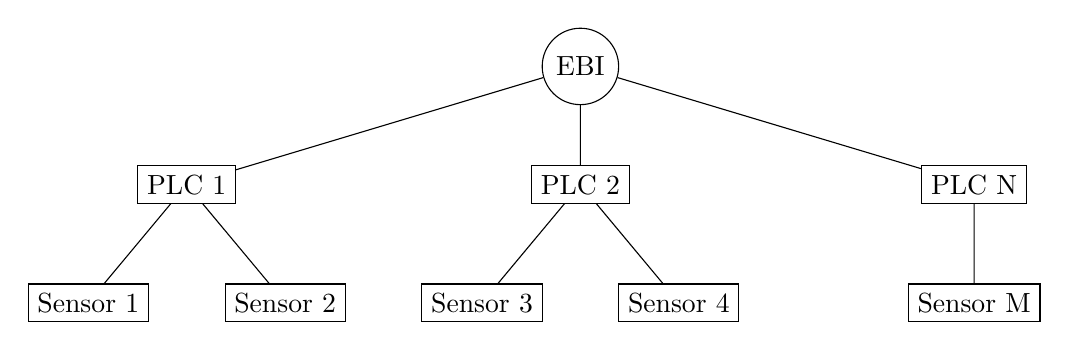
\begin{tikzpicture}[level 1/.style={sibling distance=5cm},
						level 2/.style={sibling distance=2.5cm}]
		\node[circle,draw]{EBI}
			child{
				node[rectangle,draw]{PLC 1}
					child[rectangle,draw]{node[rectangle,draw]{Sensor 1}}
					child[rectangle,draw]{node[rectangle,draw]{Sensor 2}}
				}
			child{
				node[rectangle,draw]{PLC 2}
					child{node[rectangle,draw]{Sensor 3}}
					child{node[rectangle,draw]{Sensor 4}}
				}
			child{
				node[rectangle,draw]{PLC N}
				child{node[rectangle,draw]{Sensor M}}
				}
		;
	\end{tikzpicture}
	\caption{Red industrial Gador.}
	\label{fig:redGador}
\end{figure}


\section{Introducción técnica}
\label{ch1IntroduccionTecnica}

% Presentación modelo de capas IoT
El proyecto realizado presentó una serie de desafíos a resolver, siendo el primero de ellos la variedad de tecnologías involucradas, tanto en la problemática a manipular como en la solución a implementada.
Para introducir orden en la variedad de conocimientos que forman parte del sistema desarrollado, se introduce un modelo de capas de Internet de las cosas (IoT). El modelo tiene la ventaja que separa los temas en categorías relacionadas con la función o servicio que prestan en la solución, lo que facilita su estudio. 

% Enumeración de las capas y una breve descripción de cada una
El modelo de capas seleccionado separa los conocimientos en cinco categorías, las cuales son las capas de negocio, aplicación, procesamiento, red y percepción.
La capa de negocio agrupa todo lo relacionado con las reglas y el control del sistema, esto incluye supervisar el tráfico de información, verificar el estado de los equipos u otorgar permisos a los usuarios para interactuar con el programa.
La capa de aplicación relaciona todas las tecnologías que se encargan de interactuar con el usuario final, es lo que las personas pueden ver como el sistema.
La capa de procesamiento agrupa los conocimientos cuya responsabilidad es almacenar y analizar los datos que se generan.
La capa de red tiene la finalidad de interconectar los dispositivos para permitir el flujo de datos entre todas las partes involucradas.
Finalmente la capa de percepción se refiere a todos los artefactos que manipulan o miden algo que se encuentra en el ambiente, como un sensor o un actuador. Este modelo se encuentra resumido en la tabla \ref{tab:modeloCapas}.

\begin{table}[h]
	\centering
	\caption{\label{tab:modeloCapas}Modelo de capas IoT.}
	\begin{tabular}{c c}
		\toprule
		\textbf{Capa} & \textbf{Función}                         \\
		\midrule
		Negocio       & Establecer reglas y controlar el sistema \\
		Aplicación    & Interactuar con el usuario               \\
		Procesamiento & Almacenar y analizar los datos obtenidos \\
		Red           & Transportar los datos entre dispositivos \\
		Percepción    & Realizar mediciones o acciones en planta \\
		\bottomrule
		\hline
	\end{tabular}
\end{table}

% Capa de negocios
Dependiendo del modelo viabilidad económica de un sistema y de como fue desplegado, la capa de negocio puede tener una funcionalidad contable y calcular los costos de operación.
Esta capa puede ser la encargada de determinar y generar la facturación para cobrarle a los usuarios de la aplicación, como así también, de resolver operaciones de transferencia de dinero.
La interacción en este nivel es con el personal que administra un sistema, se determina que permisos tiene cada usuario para manipular los servicios ofrecidos y se lleva adelante el registro de acciones y eventos relevantes para el normal funcionamiento del programa.

% Capa de aplicación
La experiencia que tiene el usuario al interactuar con la solución pertenece a la capa de aplicación.
Aquí se define como se presenta la interfaz gráfica que utilizan las personas, y es común utilizar un formato de sitio web.
Las páginas webs tienen la ventaja de ser indiferentes de la plataforma que utiliza el operador, solo importa que pueda ejecutar un navegador.
Actualmente, se construyen las interfaces siguiendo un modelo de diseño según el tipo de operación a realizar por el programa, si la solución abarca una interfaz hombre-máquina industrial que debe ser atendida durante toda una jornada laboral, se suele implementar una norma de manejo de situaciones anormales o ASM; si la aplicación es de uso intermitente, se puede usar un esquema de diseño material o \emph{Material Desing} que presenta una experiencia moderna y fluida, como se puede apreciar en la figura \ref{fig:ch1MaterialDesign}.
Para llevar a delante la interfaz seleccionada se utiliza un servidor que tiene como objetivo proveer los componentes gráficos al dispositivo utilizado, una manera de realizarlo es entregando al cliente una \emph{Single Web Application (SWP)}, logrando que el servidor otorgue todo el código necesario para que el dispositivo del usuario genere por si mismo los componentes gráficos a mostrar.
Es importante que el código entregado pueda ser visualizado en múltiples tamaños de pantallas, en la actualidad las personas utilizan ordenadores, tabletas y teléfonos móviles que presentan grandes diferencias en sus dimensiones, cuando una aplicación cumple con este requerimiento se dice que es responsiva.

% poner referencia de la figura en pie de página
% https://material.io/blog/mda-2020-winners
\begin{figure}[h]
	\centering
	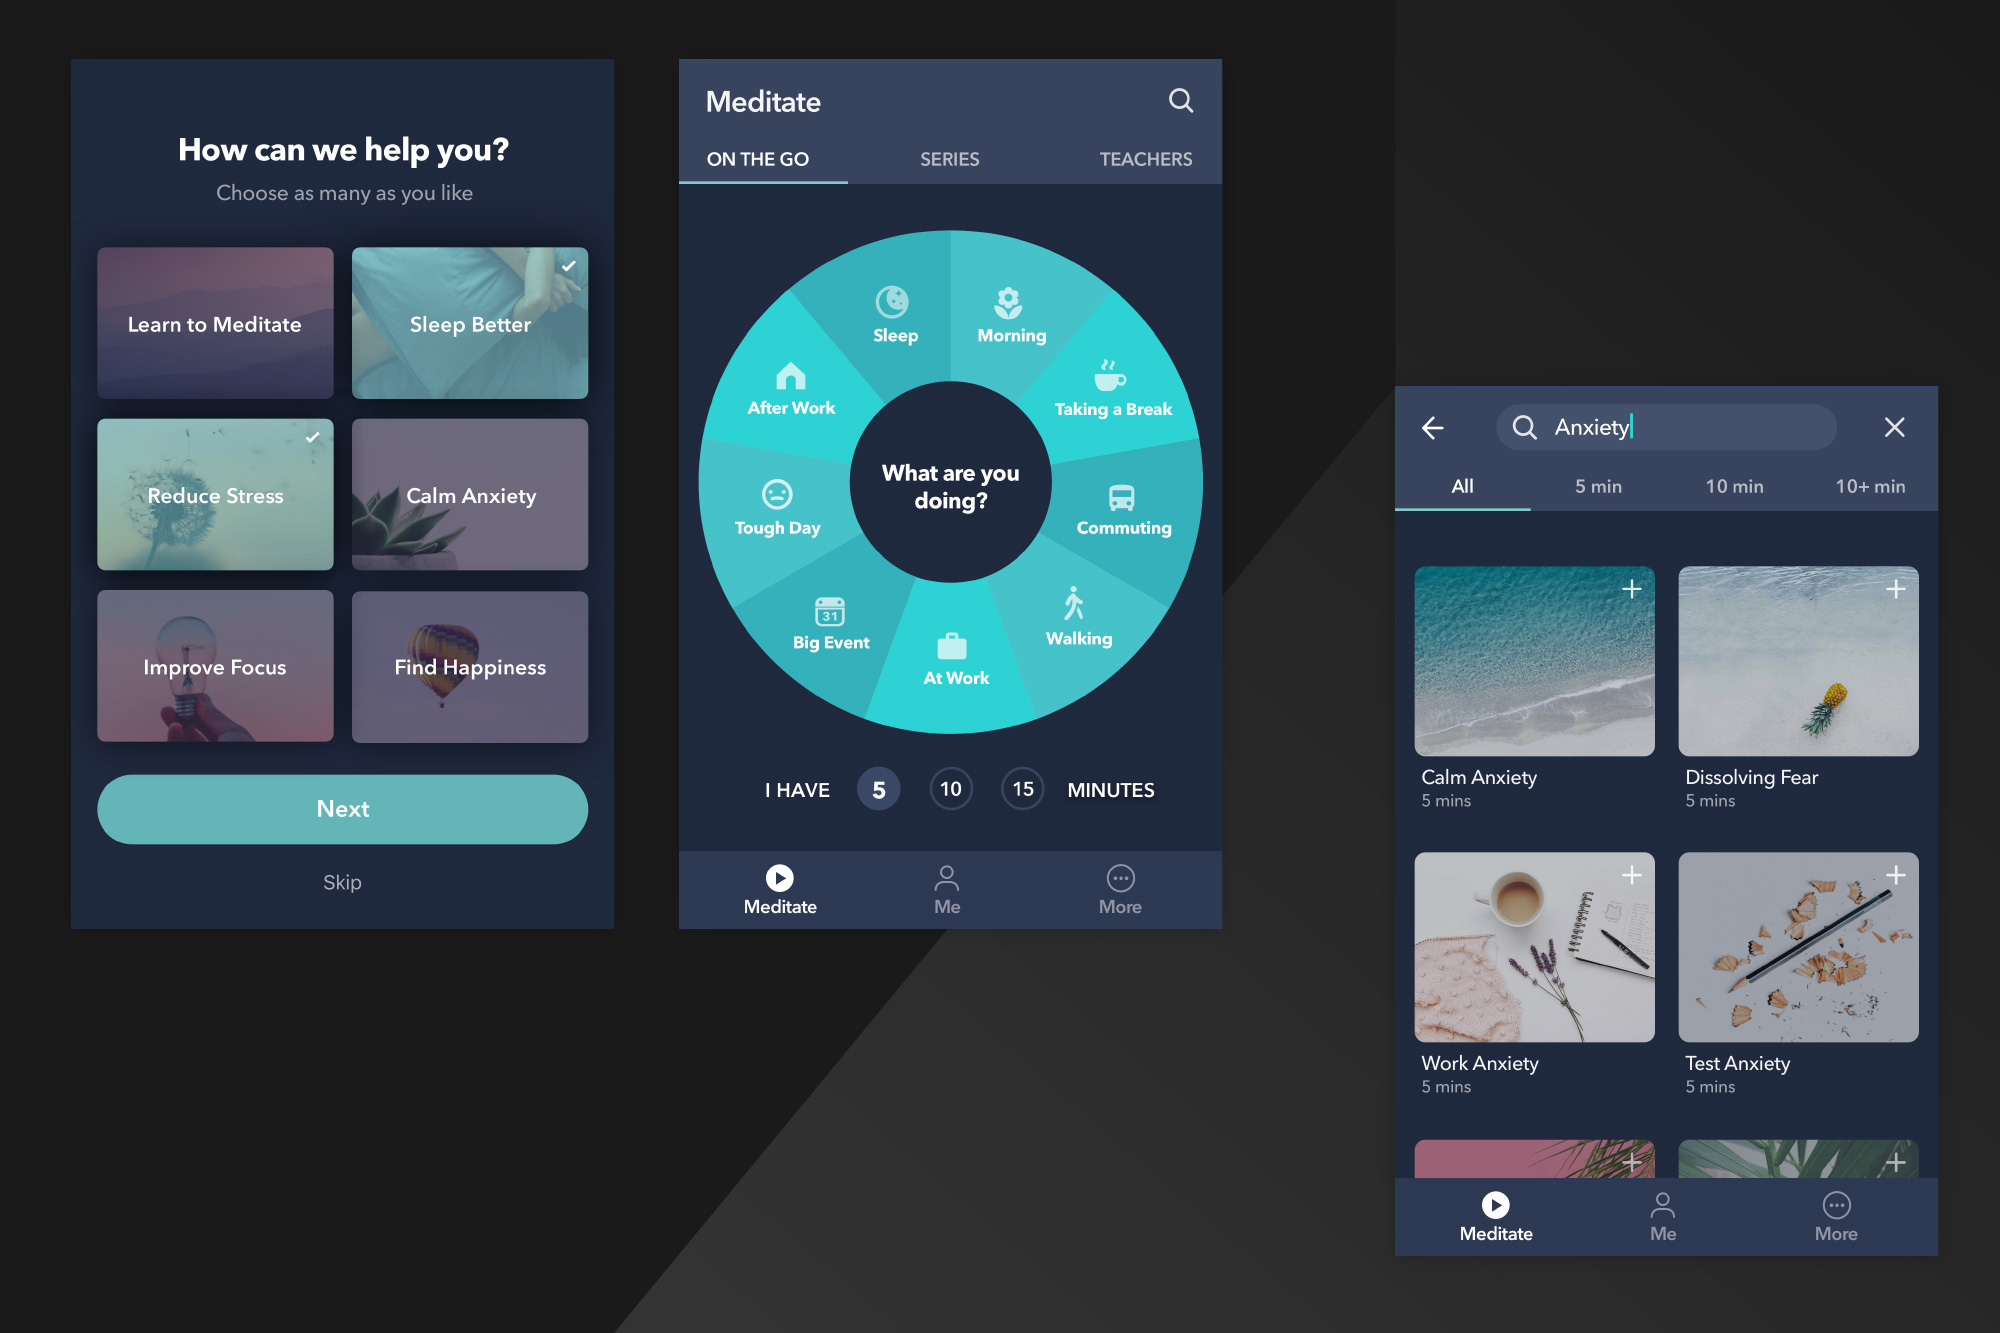
\includegraphics[width=\textwidth]{./Figures/ch1MaterialDesign.jpg}
	\caption{Ejemplo de interfaz de diseño material. \citep{WEBSITE:Material}}
	\label{fig:ch1MaterialDesign}
\end{figure}

% Capa de procesamiento
Para alimentar de datos a la interfaz gráfica se necesita de la capa de procesamiento, que entrega el contenido a mostrar en pantalla. La información puede ser almacenada con distintas tecnologías, siendo una de las principales, las bases de datos relacionales.
Este tipo de base de datos se basa en un esquema de tablas que se relacionan entre sí.
Estas tecnologías se las suelen llamar SQL, y son utilizadas principalmente en datos de inventarios y sistemas de transacciones de dinero.
Existe otro grupo de bases de datos que se denominan no relacionales o NoSQL, esta categoría contienen a las bases de datos tipo clave-valor, documental, de columnas y de grafos.

% clave-valor
Las bases de datos clave-valor tratan los datos como una única colección que puede tener campos completamente distintos en cada registro, no existe entonces, ningún tipo de relación entre los miembros de la colección. El uso principal de esta tecnología es gestionar diccionarios dentro de la memoria volátil, ya que se pueden definir tiempos de vida para los datos. La muerte programada de un dato puede ser utilizada para gestionar las sesiones de usuario dentro del programa.

% documental
Almacenar los datos de manera documental significa que se agrupa la información siguiendo un criterio de entidades similares, lo cual no significa que exista una estructura rígida, sino que los datos tienen una naturaleza similar.
La persistencia se logra siguiendo un formato de codificación estandar como \emph{XML}, \emph{YAML} y \emph{JSON}.

% columnas
Las bases de datos orientadas a columnas están pensadas para minimizar el tiempo de búsqueda, principalmente en series temporales.
La organización particular de este tipo de tecnologías es afín a los sistemas de IoT ya que los dispositivos de mediciones suelen generar un gran volumen de datos, que se pueden organizar como series temporales.

% grafos
Una base de datos orientada a grafos presenta la información como nodos que se encuentran relacionados, la diferencia fundamental con los sistemas relacionales es que los nodos no están organizados en tablas, y las relaciones que unen los nodos tienen atributos y no poseen una estructura definida.
Este tipo de tecnología permite utilizar la teoría de grafos y posibilita realizar consultas siguiendo modelos matemáticos que forman parte de esa rama de la ciencia.

% Capa de red
Se dispone de un repertorio de protocolos pertenecientes a la capa de red para lograr que los dispositivos se comuniquen entre si.
Entre los mencionados a lo largo de esta memoria se encuentran el protocolo Modbus, MQTT, HTTP y WebSocket. El manejo de estas tecnologías fue fundamental para lograr que las distintas partes del trabajo interactúen con el exterior.

% Modbus
Modbus es un protocolo que se diseñó teniendo en cuenta su uso para aplicaciones industriales, su prioridad es transmitir los datos manteniendo su integridad aún en ambientes donde el ruido eléctrico es elevado. El protocolo es público y gratuito, lo que provocó que se impusiera en un gran segmento del mercado ya que además es fácil de implementar y requiere poco desarrollo. Los dispositivos de una red Modbus tienen una dirección única y por lo general se asigna un equipo como maestro y el resto como esclavos. La arquitectura descripta presenta varias ventajas, pero la antigüedad del protocolo y su diseño para dispositivos del tipo PLC, hace que no sea adecuado para aplicaciones IoT.

% MQTT
Para interconectar a los dispositivos bajo un esquema de publicación-subscripción se utiliza el protocolo MQTT.
El protocolo está diseñado para conexiones en lugares remotos donde los dispositivos funcionan con un ancho de banda limitado.
El resultado es que los mensajes son pequeños y consumen poca batería de los equipos involucrados, por lo que se usa frecuentemente en los sistemas de IoT.
El tráfico es gestionado por un servidor del tipo broker que decide quienes son los destinatarios de un mensaje en particular, el resto de los dispositivos son clientes del broker.
Si un cliente desea transmitir datos, lo hace realizando una publicación a un determinado \emph{topic} y el broker se encarga de determinar quienes deben recibir la información enviada.
Quienes quieran obtener los datos publicados a un \emph{topic} en particular, se deben suscribir a él ante el broker.
Este al recibir una publicación de un cliente la transmite solo a los clientes que se encuentres subscritos, como se puede ver en el ejemplo de la figura \ref{fig:ch1MqttEjemplo}, donde el cliente 2 no obtiene los datos del sensor porque no se encuentra subscrito.

\begin{figure}[h]
	\centering
	\begin{tikzpicture}
		\tikzstyle{broker} = [circle,draw=black]
		\tikzstyle{publish} = [rectangle,draw=black]
		\tikzstyle{subscribe} = [rectangle,draw=black]
		\tikzstyle{flecha} = [->,very thick]

		\node[publish] (p) {Sensor};
		\node[broker,right=of p] (b) {Broker};
		\node[subscribe, right=of b] (s2)	{Cliente 2};
		\node[subscribe,above=of s2] (s1) {Cliente 1};
		\node[subscribe, below=of s2] (s3) {Cliente 3};

		\draw[flecha] (p) edge (b);
		\draw[flecha] (b) edge (s1);
		\draw[flecha] (b) edge (s3);			
	\end{tikzpicture}
	\caption{Ejemplo de comunicación MQTT.}
	\label{fig:ch1MqttEjemplo}
\end{figure}

% HTTP y Websocket
El protocolo de transferencia de hipertexto (HTTP) está orientado a transacciones y sigue el esquema petición-respuesta entre un cliente y un servidor.
El cliente inicia la comunicación enviando una petición al servidor, este último entrega una respuesta y se cierra el canal.
Existe una variante del protocolo llamada HTTPS que agrega una capa de cifrado para que las comunicaciones sean seguras.

WebSocket es un protocolo similar a HTTP pero con la diferencia que la conexión es bidireccional, esto quiere decir que cuando se logra la conectar al cliente con el servidor, ambos pueden enviar información espontáneamente. Esta cualidad permite realizar transferencias de datos en vivo, con lo que se pueden lograr servicios de \emph{streaming} o \emph{chats}.

% Capa de percepción
Los sensores utilizados en una solución de IoT están incluidos en la capa de percepción, y para que puedan formar parte del sistema se necesita que sean capaces de soportar alguno de los protocolos de comunicaciones mencionados. Dado que el desarrollo de estos dispositivos no formaron parte del proyecto realizado, no se ampliará demasiado en este tema.

% Despliegue de una solución
Teniendo definido los componentes de las capas, se necesita lograr que todas las partes funcionen como una única entidad. Para lograr este objetivo existen tecnologías de despliegue y orquestación, que cumplen la función de interconectar y mantener los servicios para que trabajen en equipo. Tradicionalmente se solían utilizar máquinas virtuales pero actualmente ese enfoque está quedando en desuso en favor de las tecnologías de contenedores. Una máquina virtual acapara parte de una computadora y funciona como un ordenador independiente, mientras que un contenedor funciona como un sistema operativo independiente pero no acapara los recursos de la computadora principal.


\section{Estado del arte}
\label{ch1EstadoDelArte}

% La nube
En la sección \ref{ch1IntroduccionTecnica} se presentó un modelo de capas para analizar las tecnologías.
En esta sección se utiliza el mismo esquema para presentar las técnicas que conforman el estado del arte.
Es importante mencionar el concepto de nube, ya que las soluciones modernas se basan en utilizar este tipo de plataforma.
La nube se refiere a utilizar servicios y servidores provistos por un tercero.
Entre los sistemas más representativos se encuentran \emph{Amazon Web Service (AWS)}, \emph{Google Cloud} y \emph{Azure}.
Estas empresas ofrecen su infraestructura y una serie de facilidades que promueven un rápido desarrollo y despliegue en el mercado.

% Percepción
Los sensores o actuadores que se utilizan corren un firmware específico para el ecosistema utilizado.
Si se decidió utilizar AWS, por ejemplo, lo más probable es que la capa de percepción ejecute \emph{AWS IoT Core} en sus dispositivos.
Este esquema es ampliamente utilizado a nivel \emph{enterprise}, por ejemplo, los laboratorios Bayer utilizan el ecosistema de AWS. \citep{WEBSITE:AWSBayer}

% Transporte
En la capa de transporte, los dispositivos se comunican usualmente utilizando los protocolos \emph{LoRaWAN}, \emph{Sigfox}, \emph{ZigBee} o \emph{Bluetooth}.
La selección del protocolo depende de las distancias a cubrir y de las necesidades energéticas.
Los sensores convergen luego a un punto de agregación.
Desde los puntos de agregación se suelen transmiten los datos al servidor en la nube utilizando el protocolo MQTT.

% Procesamiento
En la capa de procesamiento se utiliza un esquema de datos de alta disponibilidad.
Esto se logra creando réplicas de los datos en distintos servidores.
Una de las réplicas se configura como maestro y el resto como esclavos.
El servidor maestro es quien se comunica con el exterior de la réplica y retransmite los nuevos datos a los esclavos.
Si un servidor maestro sufre un problema, uno de los esclavos se convierte en el nuevo maestro y se mantiene a la réplica funcionando sin interrupciones.

Los datos pueden ser divididos en \emph{shards}, esto se hace para dividir la base de datos según la aplicación.
Un ejemplo es separar los datos por región geográfica, de esta manera los clientes de una región en particular pueden tener los servidores con los datos que suelen utilizar cerca de ellos.
Para que los \emph{shards} funcionen como una única base de datos, se dispone de un servidor \emph{router} que es la interfaz con el exterior.
El \emph{router} recibe las consultas o ingresos de nuevos datos y se encarga de utilizar el \emph{shard} correspondiente.
La configuración de este sistema se maneja desde un grupo de servidores destinados para tal fin.
Suelen conformar una réplica donde solo se almacenan los datos de configuración.
Esta arquitectura de alta disponibilidad se la conoce como granja de datos, se la puede construir con mongoDB \citep{WEBSITE:mongodbSharding} y se encuentra visualizada en la figura \ref{fig:ch1DatosAltaDisponibilidad}.

\begin{figure}[h]
	\centering
	\begin{tikzpicture}		
		\tikzstyle{block} = [rectangle,draw=black]
				
		\node[block] (r) {Router};
		
		\node[below=of r] (aux) {};
		\node[block,right=of aux] (c) {Config};
		
		\node[block,below=of aux] (s3) {Shard 3};
		\node[left=of s3] (aux1) {};
		\node[block,left=of aux1] (s2) {Shard 2};
		\node[left=of s2] (aux2) {};
		\node[block,left=of aux2] (s1) {Shard 1};
		\node[left=of s1] (aux3) {};
		
		\node[block,below=of aux3] (ra1) {Replica A};
		\node[block,below=of ra1] (ra2) {Replica B};
		\node[block,below=of ra2] (ra3) {Replica C};
		
		\node[block,below=of aux2] (rb1) {Replica A};
		\node[block,below=of rb1] (rb2) {Replica B};
		\node[block,below=of rb2] (rb3) {Replica C};
		
		\node[block,below=of aux1] (rc1) {Replica A};
		\node[block,below=of rc1] (rc2) {Replica B};
		\node[block,below=of rc2] (rc3) {Replica C};
				
		\draw (r)--(s3);
		\draw (s1)|-(c);
		\draw (s2)|-(c);
		\draw (s3)|-(aux);
		\draw (c)--(aux);
		
		\draw (ra1)-|(s1);
		\draw (ra2)-|(s1);
		\draw (ra3)-|(s1);	
		
		\draw (rb1)-|(s2);
		\draw (rb2)-|(s2);
		\draw (rb3)-|(s2);
		
		\draw (rc1)-|(s3);
		\draw (rc2)-|(s3);
		\draw (rc3)-|(s3);
	\end{tikzpicture}
	\caption{Arquitectura de datos de alta disponibilidad.}
	\label{fig:ch1DatosAltaDisponibilidad}
\end{figure}

% Aplicación
La capa de aplicación se suele diseñar rápidamente con un framework dedicado a la construcción de interfaces gráficas.
Uno de los más utilizados es Angular, desarrollado por la empresa Google.
El estilo gráfico de diseño material presentado en la sección \ref{ch1IntroduccionTecnica} es la más utilizada.
Las plataformas de nube ofrecen sus propios sistemas para diseñar la aplicación sin necesidad de escribir demasiado código, pero estas facilidades generan erogaciones adicionales.

% Negocio
La plataforma de nube presenta una capa de negocios donde se puede controlar el tráfico del sistema en ejecución.
Desde allí se puede ver la facturación estimada o el consumo de crédito para mantener en funcionamiento el proyecto.
En esta capa se pueden cambiar las variables de entorno del sistema y se pueden controlar el estado de los componentes.
Es posible montar servicios que corran programas como \emph{Checkmk} o \emph{Grafana} para visualizar el estado de los dispositivos en campo. O se puede optar por usar los servicios que ofrezca la empresa de nube.

% Orquestación y despliegue
La tecnología que se suele utilizar para orquestar toda la solución es Kubernetes, ya que además de automatizar el despliegue, también permite ajustar la escala.
Ajustar la escala se refiere a la capacidad de crear una réplica de un servicio cuando uno de ellos está trabajando cerca de su límite de procesamiento.
Es un sistema basado en contenedores y crea un \emph{clúster} a partir de una plantilla donde se definen las reglas de escalamiento.

\section{Objetivos y alcance}
\label{objetivos}

% Objetivos
El objetivo principal que cumplió este proyecto fue demostrarle al cliente el potencial de las nuevas tecnologías y la posibilidad de integrarlas a sus actuales sistemas.
Se propuso crear una prueba de concepto para evaluar la viabilidad de futuros proyectos.
La creación de un sistema que pueda unir equipos que utilizan Modbus con aquellos que usan MQTT, es de relevancia en general para la industria local.
Otro objetivo importante fue la de utilizar las técnicas adquiridas durante la cursada de la especialización.
Con la finalidad de sementar los conocimientos a través de la práctica.

% Alcance
El proyecto se limitó a desarrollar el software a desplegar en un servidor que fue nombrado Nodos.
Esto significa que no se contempló el desarrollo del hardware, en particular los sensores y los puntos de agregación.
E esquema del servidor en la red de Gador puede ser visualizado en la figura \ref{fig:esquemaProyecto}.
El servidor puede comunicarse con EBI de la misma manera que lo logra un PLC.
Además tiene la capacidad de utilizar el protocolo MQTT para conectarse directamente con los sensores o a través de puntos de agregación.


\begin{figure}[h]
	\centering
	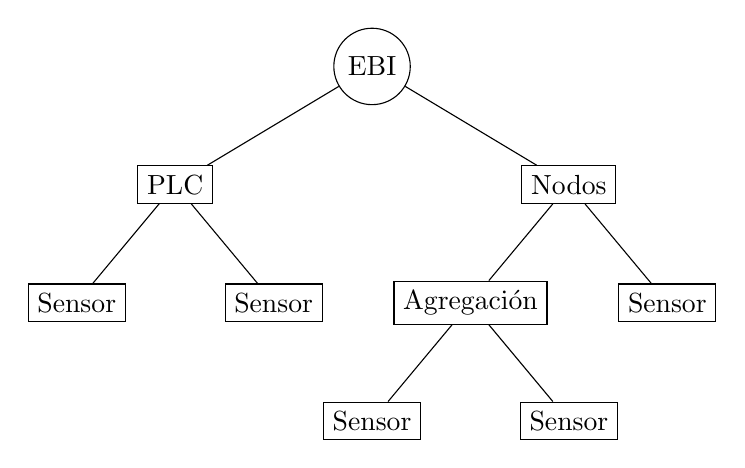
\begin{tikzpicture}[level 1/.style={sibling distance=5cm},
						level 2/.style={sibling distance=2.5cm}]
		\node[circle,draw]{EBI}
			child{
				node[rectangle,draw]{PLC}
					child[rectangle,draw]{node[rectangle,draw]{Sensor}}
					child[rectangle,draw]{node[rectangle,draw]{Sensor}}
				}
			child{
				node[rectangle,draw]{Nodos}
					child{
						node[rectangle,draw]{Agregación}
							child[rectangle,draw]{node[rectangle,draw]{Sensor}}
							child[rectangle,draw]{node[rectangle,draw]{Sensor}}
					}
					child{node[rectangle,draw]{Sensor}}
				}
		;
	\end{tikzpicture}
	\caption{Red industrial Gador.}
	\label{fig:esquemaProyecto}
\end{figure}

% Requerimientos
Cuando se tuvo definidos los objetivos y el alcance del proyecto, se inició un proceso de negociación con el cliente.
Se buscó determinar cuales eran sus necesidades y sus temores respecto del proyecto.
Las conversaciones con el cliente dieron como resultado la siguiente lista de requerimientos:

\begin{itemize}
	\item Debe integrarse a la infraestructura de Gador S.A. sin generar conflictos en otros sistemas.
	\item Debe crear tramas en el formato \emph{Enterprise Buildings Integrator} y enviarlas al servidor.
	\item Debe interpretar eventuales mensajes del servidor \emph{Honeywell}.
	\item Debe interpretar los mensajes de los sensores.
	\item Debe poder cambiar la frecuencia de lectura de mediciones.
	\item Debe poseer la capacidad de gestionar los ingresos de usuarios de forma segura.
	\item Debe permitir que por lo menos cinco usuarios accedan al sistema simultáneamente.
	\item Debe presentar una interfaz donde se monitoree el estado de los sensores
	\item Debe permitir elegir un sensor en particular para editarlo.
	\item Debe poseer un módulo de gestión de usuarios.
	\item Debe ser compatible con ordenadores de escritorio y smartphones.
	\item Las contraseñas no persistirán como texto plano.
	\item Debe persistir todas las modificaciones realizadas a la configuración de los sensores.
	\item Debe persistir las mediciones obtenidas.
\end{itemize}